%% -*- coding: utf-8-unix -*-

\chapter{NetTesterの技術仕様}
\label{chap:nettester-design}

 \section{NetTesterのモデル}
 \label{sec:nettester-model}

 \subsection{基本的な構成要素}
%  NetTester の構成(モデル)
% つかっている技術:
% \begin{itemize}
%  \item network namespaceとその操作, trema/phut
%        \begin{itemize}
%         \item Phut Memo – NetTester \url{https://3.basecamp.com/3088280/buckets/867009/documents/238439817}
%        \end{itemize}
%  \item patch panel 実装, ActiveFlow
%        \begin{itemize}
%         \item パッチの概要 → パッチ – NetTester \url{https://3.basecamp.com/3088280/buckets/867009/documents/213266851}
%         \item "patch panel" model – NetTester \url{https://3.basecamp.com/3088280/buckets/867009/documents/208275139}
%        \end{itemize}
% \end{itemize}
% phut, activeflowなどの実装寄りのはなしは付録とかにするか。

本プロジェクトでは、\ref{sec:basic-tester-idea}節で解説したネットワーク
テストシステムのアイディアを、NetTester~\cite{nettester}というツールとし
て実装した。NetTester は\figref{fig:model-nettester}の示すコンポーネント
で構成される。

\begin{figure}[h]
 \centering
 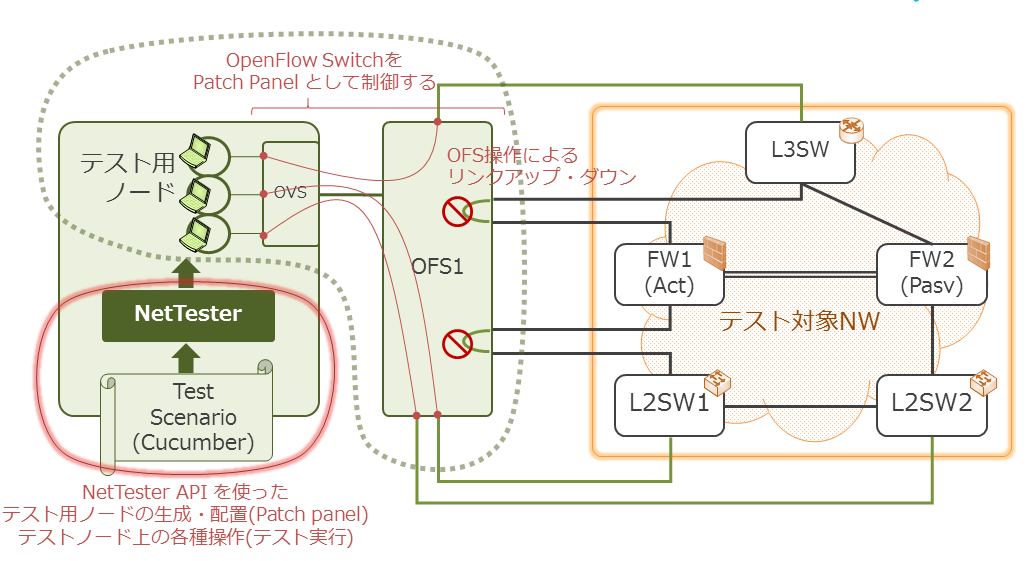
\includegraphics[scale=0.6]{img/model-nettester.png}
 \caption{NetTesterのモデル}
 \label{fig:model-nettester}
\end{figure}

% TODO: PSW, SSWなどの用語にもとづいて図の中身を修正すること

\begin{description}
 \item[物理スイッチ(OFS)] パッチパネルとして動作させるOpenFlowスイッチ
            \footnote{本書あるいはNetTester関連ドキュメント中では ''物理
            OpenFlowスイッチ'',``Physical (OpenFlow) Switch'',''PSW''な
            どで表記される。}。テスト対象ネットワークのトポロジ操作やテ
            スト用ノードの配置などをおこなう、物理ポートを複数もつスイッ
            チである。
 \item[ソフトウェアスイッチ(OVS)] パッチパネルとして動作させるOpenFlowス
            イッチ\footnote{本書あるいはNetTester関連ドキュメント中では、
            ``Software (OpenFlow) Switch'',''SSW''などで表記される。ある
            いは、実装上はOpen vSwitchを使用していることから、単に''OVS''と
            することがある。}。仮想ノードとして作成したテスト用ノードを
            収容し、物理スイッチを介してテスト対象ネットワークにノードを
            配置するためのスイッチである。
 \item[テスト用ノード] テスト対象ネットワークのふるまいを調べるために、
            テストトラフィックを生成しするためのノード。実装としては、
            Linux OS 上の仮想ノード(Linux Network Namespaceを使用したノー
            ド)で実現される。
 \item[NetTester] テスト用ノードやパッチパネルの作成・管理・制御をおこな
            うためのツール。テストシナリオを実行するために必要なテスト用
            リソース(テスト用ノードとパッチによる配置)操作のためのAPIを
            提供する。
 \item[NetTester Server(Linux)] NetTester を実行し、テスト用ノードをホス
            トするサーバ。Network Namespace が利用可能な Linux OS を使用
            する。
 \item[テストシナリオ] テスト対象ネットワークのふるまいをしらべるための
            手順(シナリオ)定義。本プロジェクトではCucumberを使ってテスト
            シナリオの記述・実装をおこなう。
\end{description}

\subsection{構成上の制限・制約}
現時点(2016年1月)のNetTesterでは\figref{fig:model-nettester}のとおりにモ
デルを定義している。このモデル定義から、以下のようなテストシステム構成上
の制限や制約がある。
\begin{itemize}
 \item NetTester が制御可能な物理スイッチはひとつだけである。そのため、
       テスト対象ネットワークで操作可能なリンクやテスト用ノード配置可能
       な範囲は物理スイッチの持つポート数を上限として制限される。
 \item NetTester が制御可能なソフトウェアスイッチはひとつだけである。ま
       た、NetTester は NetTester が実行されるOS上でのみテスト用ノードの
       生成・操作ができる。
 \item 物理スイッチおよびソフトウェアスイッチを接続するためのリンクは1本
       とし、物理スイッチ側のポート番号をPort 1とする。
       %% TODO: 詳細は後述 → フロー設計あたりか?
       また、このリンクはNetTesterを実行するで専有して使用する。
       (NetTester Server を仮想マシンとして実行する場合、PSW-SSWを接続す
       るための物理リンク/物理ポートを他の仮想マシンと共有させない。)
       %% TODO: Tester Set の定義をどこかにいれるべき?
\end{itemize}
これらのモデル定義および制限の設定は、NetTester 実装をシンプルにするため
のものである。本プロジェクトでは、NetTester それ自体の機能拡張や拡張性の
担保ではなく、BDDベースのネットワークテスト(ユースケースの実証)を目標と
している(\ref{sec:behavior-test}節参照)。

\section{フロールール設計}

2015年度実装に対してあるていど簡略化した実装になっているのでそのへんのはなし。
flowの優先度
\begin{itemize}
 \item テスト対象NW→Host(テストノード)へのbroadcastのコントロール – NetTester \url{https://3.basecamp.com/3088280/buckets/867009/todos/198950295}
 \item NetTester機能拡張検討
       \url{https://drive.google.com/file/d/0B2eRR_JxYJA5TmhaeWItNF93Um8/view}
       いくつのフロー案とどれを、なぜ選択したのか、という話
 \item Table \& Rule Priority Design (2015 ool-l1patch) – NetTester \url{https://3.basecamp.com/3088280/buckets/867009/documents/211290387}
 \item Table \& Rule Priority Design (NetTester) – NetTester \url{https://3.basecamp.com/3088280/buckets/867009/documents/217426690}
       \begin{itemize}
        \item default deny の要否: packet-in をいれるかどうか → デバッグ用途のはなし?
        \item packet-in による trema の trouble/trouble shoot → 補足とかでいれる?
              \begin{itemize}
               \item 謎PacketInで死なずにログを出す – NetTester \url{https://3.basecamp.com/3088280/buckets/867009/todos/221324759}
               \item 調査: テスト環境でOFS(Pica8)-OFC(NetTester/Trema)の接続が切れる – NetTester \url{https://3.basecamp.com/3088280/buckets/867009/todos/218484578}
              \end{itemize}
       \end{itemize}
 \item VLAN Trunk Portを使ったテストシナリオを作る – NetTester \url{https://3.basecamp.com/3088280/buckets/867009/todos/238166429}
 \item テスト対象NW機器間接続patch機能を作る – NetTester \url{https://3.basecamp.com/3088280/buckets/867009/todos/238169839}
\end{itemize}

\section{リンク操作方式}

\begin{itemize}
 \item テスト対象NW機器間接続のup/down方式を決める – NetTester \url{https://3.basecamp.com/3088280/buckets/867009/todos/238171702}
 \item リンクダウン・リンクアップ機能用のスクリプト実装 – NetTester \url{https://3.basecamp.com/3088280/buckets/867009/todos/247379766}
\end{itemize}

\section{制限・制約}

フロールールから: arp があるていどみえてしまうこと → セキュリティについて?

DPIDや一部のポート番号の固定について
\begin{itemize}
 \item NetTesterの実装で気になるところ – NetTester \url{https://3.basecamp.com/3088280/buckets/867009/todos/196940380}
\end{itemize}

NetTester 自体の通信要件?
\begin{itemize}
 \item openflow, ssh, syslog 等
\end{itemize}


%%% Local Variables:
%%% mode: yatex
%%% TeX-master: main.tex
%%% End:
